\section{Experimental Apparatus}
\label{sec:exp apparatus}

\begin{figure*}
\begin{center}
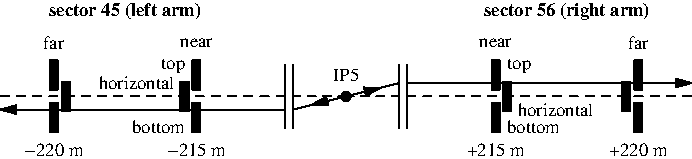
\includegraphics{fig/elastic_principle.pdf}
\hfil
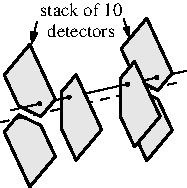
\includegraphics{fig/stationScheme.pdf}
\caption{%
Left: schematic view of the RP stations on both sides of IP5 with two proton tracks from an elastic event. Right: Schematic view of the silicon detector positions in an RP station with a track traversing the overlap zone between top and horizontal detectors, providing detector alignment information. 
}
\label{fig:rpsketch}
\end{center}
\end{figure*}

The TOTEM experiment, located at the LHC Interaction Point (IP) 5 together with
the CMS experiment, is dedicated to the measurement of the total 
cross-section, elastic scattering
and diffractive processes. The experimental
apparatus, symmetric with respect to the IP, is 
composed of a forward proton spectrometer (Roman Pots, RPs) and the 
forward tracking telescopes T1 and T2. 
A complete description of the TOTEM detector instrumentation 
and its performance is given in~\cite{totem-jinst} and~\cite{totem-ijmp}. 
The data analysed here come from the RPs only. An RP is a movable beam-pipe
insertion capable of approaching the LHC beam to a distance of less than a millimeter, in 
order to detect protons with scattering angles of only a few microradians. 
The proton spectrometer is organised in two RP stations: one on the left side of the IP 
(LHC sector 45) and one on the right (LHC sector 56), see Figure~\ref{fig:rpsketch} (left).
Each RP station, located between 215 and 220\,m from the IP, is composed of two 
units: ``near'' (215\,m from the IP) and ``far'' (220\,m). 
A unit consists of 3 RPs, one
approaching the outgoing beam from the top, one from the bottom, and one 
horizontally.
Each RP houses a stack of 10 silicon
strip detectors designed with the specific objective of
reducing the insensitive area at the edge facing the beam
to only a few tens of micrometers. Due to the 5\,m long lever arm 
between the near and the far RP units 
the local track angles can be reconstructed
with a precision of about $10\,\mu$rad. A high trigger efficiency
($> 99$\%) is achieved by using all RPs independently. 
Since elastic scattering events consist of two collinear protons emitted in 
opposite directions, the detected events can have two topologies, called 
diagonals: 45 bottom -- 56 top and 45 top -- 56 bottom.

This article uses a reference frame where $x$ denotes the horizontal axis (pointing out of the LHC ring), $y$ the vertical axis (pointing against gravity) and $z$ the beam axis (in the clockwise direction).
